\documentclass[english,oribibl]{llncs}
\usepackage[T1]{fontenc}
\usepackage[latin1]{inputenc}
\usepackage{babel}
\usepackage{times}
\usepackage{graphicx}
\usepackage[a4paper, tmargin=2.5cm, bmargin=2cm, lmargin=2.5cm, rmargin=2.5cm,nohead]{geometry} 
\usepackage{listings}
\lstset{keywordstyle=\bfseries, flexiblecolumns=true}
\lstloadlanguages{[ANSI]C,[ANSI]C++,HTML}
\lstdefinestyle{prg} {basicstyle=\small\sffamily, lineskip=-0.2ex}
\lstdefinestyle{inlineprg} {basicstyle=\small\sffamily}

\newcommand{\fig}[3][htbp]{ % text => 10pt helvetica
  \begin{figure}[#1] {\centering{\includegraphics[scale=0.5]{fig/#2}}\par}
    \caption{#3\label{fig:#2}}
  \end{figure}
}

\newcommand{\prg}[4][htbp]{
  \begin{figure}[#1]
    \vspace{\parskip}
    \makebox[\textwidth][c]{
      \lstinputlisting[language=#2,style=prg]{prg/#3.prg}}
    \vspace{0.5\parskip}
    \caption{#4\label{prg:#3}}
  \end{figure}
}

\newcommand{\prgbox}[4][htbp]{
  \begin{figure}[#1]
    \vspace{\parskip}
    \framebox[\textwidth][c]{
      \lstinputlisting[language=#2,style=prg]{prg/#3.prg}}
    \vspace{0.5\parskip}
    \caption{#4\label{prg:#3}}
}

\newcommand{\inlineprg}[2][C++]{
  \vspace{\parskip}
  \noindent\makebox[\textwidth][c]{
    \begin{lstlisting}[language=#1,style=inlineprg]{}
      ^^J #2
    \end{lstlisting}}
  \vspace{0.5\parskip}
}

\def\textprg{\lstinline[language=C++,style=inlineprg]}

\title{\textsc{Epos}-MPI: a highly configurable Run-time System for Parallel Applications}
\author{
  Andr� Lu�s Gobbi Sanches and Ant�nio Augusto Fr�hlich\\
  UFSC/CTC/LISHA\\
  PO Box 476\\
  88049-900 Florian�polis - SC, Brazil\\
  \texttt{\{gobbi,guto\}@lisha.ufsc.br}\\
  \texttt{http://www.lisha.ufsc.br/$\sim$\{gobbi,guto\}}
}
\date{}

\bibliographystyle{plain}

\begin{document}
\maketitle
\thispagestyle{empty}

\begin{abstract}
 
  This paper presents an implementation of MPI over a highly
  configurable operating system, \textsc{Epos}. By using the advanced
  features of \textsc{Epos} Communication system, MPI was implemented as
  a thin layer instead of a \emph{middleware} library. The design is
  based on the Application Oriented System Design methodology, and
  static metaprogramming, generic programming and aspect orientation
  were applied in the implementation.
  
  MPI collective operations are decomposed in 3 entities, simplifying
  their implementations and allowing them to be ported to other
  message-passing systems.

  \paragraph{Keywords:} application-oriented operating systems, 
  generic programming, aspect oriented, static metaprogramming, MPI,
  collective communication.
  
\end{abstract}

%%%%%%%%%%%%%%%%%%%%%%%%%%%%%%%%%%%%%%%%%%%%%%%%%%%%%%%%%%%%%%%%%%%%%%%%%%%%%%%
\section{Introduction}

% - Motivation for clusters + MPI
%   - Effective alternative to custom distributed memory architectures (MPP)
%   - MPI: supercomputer API on NOWs -> boosted the cluster revolution
%   - SMP: multithreading X MPI -> orthogonal
The \emph{Message Passing Interface}~(MPI)~\cite{MPI_1_1} standard
played a major role for the dissemination of parallel programming. Being
a \emph{de facto} standard in the filed, with implementations for
virtually any distributed-memory parallel machine, MPI was one of the
main factors that stimulated the cluster computing phenomenon of recent
years. As ordinary desktop operating systems begun to figure MPI
implementations, it became possible for numerous parallel applications,
originally developed for supercomputers, to be executed in low-cost
clusters of commodity workstations. Moreover, the availability of a
common API for message passing programming encouraged the development of
several new parallel applications.

% - The commodity discussion
%   - Some cluster people insist in extending the commodity concept to the
%     software, but ordinary OS (Unix, Windows) were conceived to support
%     interactive, graphical, web-aware applications, whereas supercomputers
%     always used specialized RTSS (cite PUMA, PEACE, UNICOS, IBM-MPI, etc)
%   - Those compromised with high-performance are doing OS-bypass, thus
%     recognizing the call for custom software
Other nuisances of the cluster computing phenomenon are not so
straightforward, however. For instance, most people have ``commodity
hardware'' as an axiom of cluster computing and ``commodity software''
as a corollary. By analyzing the question in depth, one will easily
conclude that what we now call ``commodity hardware'' could very well
be called ``supercomputing hardware'' ten years ago: commodity
processors now feature multiple functional units that operate in
parallel; commodity memory hierarchies now deliver amazing storage
capacity and bandwidth; and commodity high-speed networks now operate at
speeds close to internal busses.  Indeed, what happened was a
convergence of desktop computer hardware toward high-performance.

Notwithstanding, the reasoning presented above fails when applied to
``commodity software''. As of today, commodity desktop system software
can be summarized in two families: \textsc{Unix} and \textsc{Windows}.
Both families have been developed to support interactive, graphical,
web-aware applications. In contrast, looking behind the front-end of a
supercomputer one is likely to find a highly specialized operating
system, designed and implemented to satisfy the heavy demands of
parallel applications~\cite{Wheat:1994, Preikschat:1994a}. There is no
convergence foreseeable in this area, since parallel run-time support
systems are way too specialized to support an all-purpose desktop.
Indeed, several MPI implementations for clusters of workstations rely on
communication subsystems that bypass the host operating system to
directly access the interconnection hardware~\cite{Lumetta:1997,
  Tezuka:1997, Prylli:1998}.  This is the most evident recognition that
commodity system software is not adequate to support parallel computing
on clusters of workstations.

% - The true story of MPI
%   - Just an API that can be mapped onto any parallel (distributed memory)
%     operating system
%   - Room to take advantage of special architectural features, such as the
%     built-in processor in Myrinet and the global addres space in SCI
In fact, MPI is a standard \emph{interface} that was idealized to be
implemented on top of a native communication system. The inability of
ordinary operating systems to deliver an adequate communication system
made room for complex \emph{middleware} implementations that override
much of the native communication system~\cite{Gropp:1996:HPI,
  burns94:_lam, squyres03:_compon_archit_lam_mpi}. These middleware
implementations are far from ideal, for they aggregate unnecessary
overhead and usually fail to explore particularities of both run-time
system and interconnection hardware. For instance, some high-speed
networks feature their own processor and could operate as an asymmetric
multiprocessor with the main processor(s), implementing most of what is
needed to deliver an MPI-compliant communication system. This would be
impracticable with a middleware implementation.

% - Software engineering
%   - If MPI is only an API and we can freely design and implement our parallel
%     RTSS, then let's do it on modern SE basis instead of deploying the ADI
%     (or channel) concept of MPI-CH (which is a GOOD compromise for porta-
%     bility, but far from other SE metrics)
%   - AOSD -> break the monolithic design to model the RTSS as families of
%     abstractions with members that are specialized to particular classes of
%     parallel applications
%   - AOOS MPI
%   - \textsc{Epos}-MPI 
Nevertheless, if MPI is nothing but an interface, exporting the
functionality of a parallel run-time environment ---designed and
implemented according to modern software engineering techniques--- in a
way that complies with the standard should be straightforward.
Furthermore, it could reveal novel alternatives to handle important
aspects such as group communication, collective operations, and data
encapsulation. In this scope, this article presents an implementation of
MPI based on the \emph{Application-Oriented System Design} method
proposed by Fr�hlich~\cite{Frohlich:2001}. The main idea is to produce a
set of software components that are able to efficiently bridge a
preexisting communication system to the MPI standard, taking in
consideration the specific requirements of particular applications.  The
substratum for this work is the communication system of the
\emph{Parallel Embedded Operating
  System}~(\textsc{Epos})~\cite{EPOS_Myri}, which is based on the
\textsc{Myrinet} high-speed network~\cite{boden95Myrinet}.


% - Article
%   - Structure
The remainder of this article is organized as follows: section section
\ref{sec:traditional} describes the structure of a traditional MPI
implementation; sections \ref{sec:design} \ref{sec:epos-mpi} describe
the presented implementation and compares its performance to another MPI
implementation; section \ref{sec:related} lists related work; and
section \ref{sec:conclusions} is this paper conclusion.

%\section{Network Topologies} \label{topologies}

%        The following figures illustrate the network topologies most found in parallel systems.


%        \bigskip

%%\begin{figure}[h]
%        \centerline{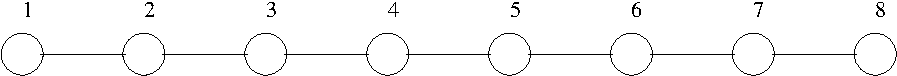
\includegraphics[scale=0.5]{pictures/top_linear.pdf}}
%        \medskip
%        \centerline{Linear Topology}
%        \bigskip
%        %\caption{Linear Topology}
%        %\label{fig::top_linear}
%%\end{figure}

%%\begin{figure}[h]
%        \centerline{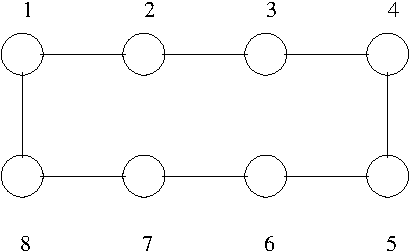
\includegraphics[scale=0.5]{pictures/top_circular.pdf}}
%        \medskip
%        \centerline{Ring Topology}
%        \bigskip
%%       \caption{Ring Topology}
%%       \label{fig::top_circular}
%%\end{figure}

%%\begin{figure}[h]
%        \centerline{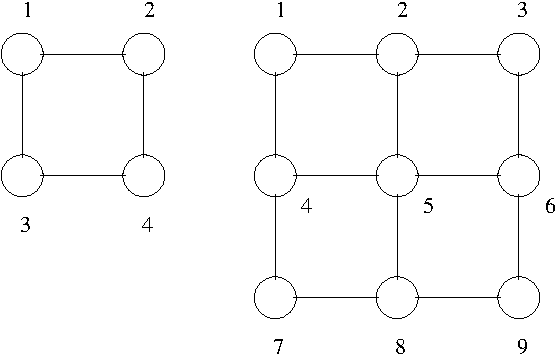
\includegraphics[scale=0.5]{pictures/top_mesh.pdf}}
%        \medskip
%        \centerline{Mesh Topology}
%        \bigskip
%%       \caption{Mesh Topology}
%%       \label{fig::top_mesh}
%%\end{figure}

%%\begin{figure}[h]
%        \centerline{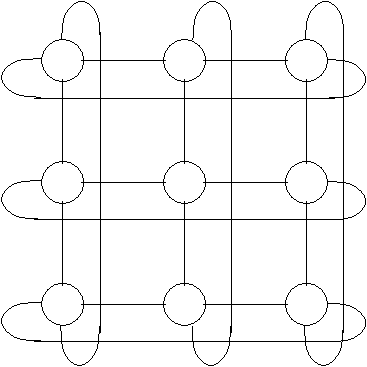
\includegraphics[scale=0.5]{pictures/top_torus.pdf}}
%        \medskip
%        \centerline{Torus Topology (bidimensional)}
%        \bigskip
%%       \caption{Torus Topology (bidimensional)}
%%       \label{fig::top_torus}
%%\end{figure}

%%\begin{figure}[h]
%        \centerline{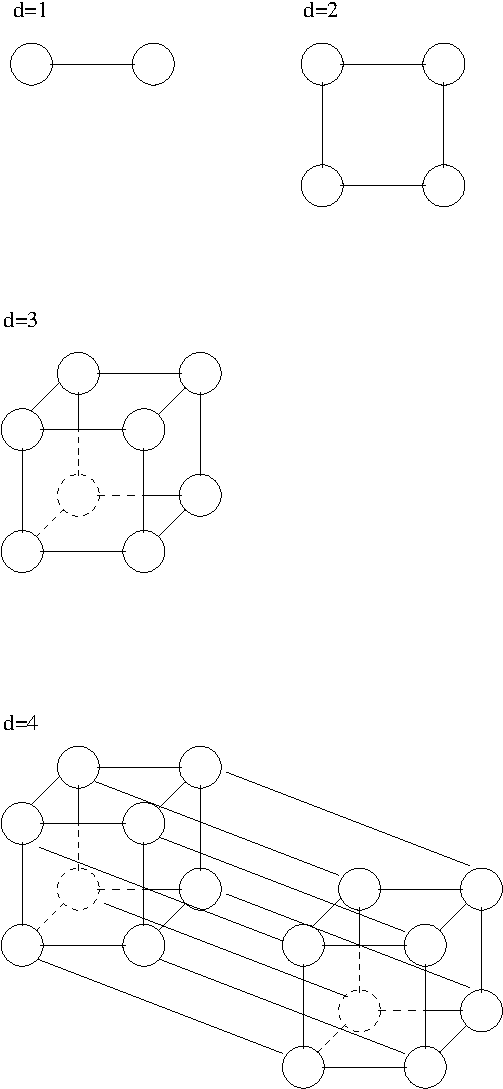
\includegraphics[scale=0.5]{pictures/top_hipercubo.pdf}}
%        \medskip
%        \centerline{Hypercube Topology}
%        \bigskip
%%       \caption{Hypercube Topology}
%%       \label{fig::top_hipercubo}
%%\end{figure}

%%\begin{figure}[h!]
%        \centerline{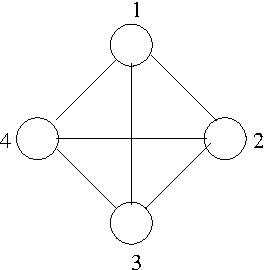
\includegraphics[scale=0.5]{pictures/top_completa.pdf}}
%        \medskip
%        \centerline{Complete Topology}
%        \bigskip
%%       \caption{Complete Topology}
%%       \label{fig::top_completa}
%%\end{figure}

%\section{Software Engineering} \label{engsoft}

%\subsection{Static Metaprogramming}

%        Metaprogams are programs which manipulate programs. The input of a metaprogram may be another program or the metaprogram itself. Compilers and preprocessors are examples of metaprograms. Static metaprograms are programs which run before the programs they manipulate.

%        The C++ language offers static metaprogramming through template metaprogramming. Class templates may be defined, which can be instanciated by supplying the parameters on which the class is generic. An example follows:

%\begin{verbatim}

%template<class T> class C {
%        T t;
%public:
%        ...
%        inline T& operator+= (T _t) {
%                t += _t;
%                return (*this);
%        }
%        ...
%};

%int i;
%C<int> ci;
%C<char> cc;
%C< C<int> > cci;

%\end{verbatim}

%        In the example, the \verb!C! class is defined as a template which is generic on its parameter class \verb!T!. \verb!T! can be any type, as long as it provides the operator \verb!+=!, which is used. For each value that the parameter \verb!T! undertakes (\verb!int!, \verb!char!, \verb!C<int>!) a new class will be generated based on the template. The generated code of a template instantiation is identical to the code of a normal class. Recursive template instantiation (\verb!C< C<int> >!) is allowed since the \verb!C! template class provides every operator required (the \verb!+=! operator).

%        The \verb!inline! directive used means that calls to the functions should be replaced by its contents. Thus calling \verb!ci += 3;! or \verb!i += 3;! generate exactly the same code, with no performance overhead.

%\subsection{Generic Algorithms} \label{iteradores}

%        Algorithms can be parametrized in order to be generic. These algorithms are compatible with any type which provides the necessary operators. The C++ standard library provides a set of containers and generic algorithms that can iterate through any container. Each container provides an Iterator class, which references its elements. Generic algorithms only access containers through its iterators, whose common interface is stated by the standard, and so the containers' implementation is hidden.

%        An iterator may be a pointer, an index or even a class. The use of an iterator doesn't change performance, thanks to static metaprogamming. Further discussion on containers and iterators can be found in \cite{Stroustrup:1997}.

%% Aspect Oriented Programming
%Aspect-Oriented Programming (AOP) was introduced by Kiczales [KLM+97] to deal with non-functional properties of component-based systems. Most of the current component-based development strategies concentrate on defining and composing functional units, and do not properly address the representation of non-functional properties captured during system design. In these strategies, properties such as synchronization, error handling, and security are usually expressed as small code fragments scattered over several components. Developing and maintaining such a kind of entangled code constitutes one of the biggest problems in component-based software engineering, because it ruptures with important concepts like encapsulation and cohesion and compromises the software quality. Furthermore, a component that is hardwired to a specific environment will hardly be reused in another. Aspect-oriented programming captures non-functional properties in reusable units called  aspects . Aspects are specified in aspect-oriented languages and woven with components by aspect weavers to generate the target system. This process of combining aspects and components is instrumented by join points, which are elements of the component language semantics understood by the aspect program and used for coordination.

%        In the \textsc{Epos} operating system, aspects are implemented using template metaprogramming.

%% \textsc{Epos}
%Domain engineering methodologies that drive the design process toward
%collections of reusable software components are largely used in the
%realm of applicative software. Recently, strategies to develop
%component-based operating systems begun to
%appear~\cite{Baum:1999,Constantinides:2000,Frohlich:2001} and are
%producing exciting new operating systems such as
%\textsc{Epos}~\cite{Frohlich:2001} and \textsc{Pure}~\cite{Schoen:1998}. Being fruit of
%a domain engineering process (instead of a system engineering process),
%the software components of such systems can be arranged to build a large
%variety of run-time support systems. More specifically, the
%\emph{Application-Oriented System Design}~(AOSD) method proposed by
%Fröhlich~\cite{Frohlich:2001} combines principles of
%\emph{Object-Oriented Design}~(OOD)~\cite{Booch:1994} with
%\emph{Aspect-Oriented Programming}~(AOP)~\cite{kiczales97aspectoriented} and
%\emph{Static Metaprogramming}~(SMP)~\cite{Czarnecki:2000} in a method
%that guides the development of highly adaptable software components for
%the operating systems domain.

%% \textsc{Epos} Communication System
%\subsection{\textsc{Epos} Communication System}

%        The \textsc{Epos} Communication System is composed by four entities: Communicator, Channel, Network and Envelope. Application processes communicate with each other using the \emph{Communicator}, which acts as an interface for a communication \emph{Channel} implemented over a \emph{Network}. The messages sent over a \emph{Communicator} can be specified as sequences of bytes of known length, or they can be covered by an \emph{Envelope}.

%        The \emph{Channel} abstraction handles network independent transport details (OSI layer 4). Network details are handled by the \emph{Network} abstraction, which provides a uniform view of networks to the \emph{Channel}.  The \emph{Envelope} abstraction represents messages. It deals with notation conversions and is also responsible for zero copy transfers.

%        Applications interact only with the \emph{Communicator} and the \emph{Envelope} abstraction. \emph{Envelopes} are initialized with the contents of the message to be transferred and sent to a \emph{Communicator}.


%%%%%%%%%%%%%%%%%%%%%%%%%%%%%%%%%%%%%%%%%%%%%%%%%%%%%%%%%%%%%%%%%%%%%%%%%%%%%%%
\section{Typical MPI Implementations\label{sec:traditional}}

% - Typical designs are monolithic
%   - A single software architecture, with single generic functional units
There are basically two approaches that have been used to implement
MPI\cite{Gropp:1994}: specialized libraries optimized for a given
parallel machine~\cite{cray, ibm}, or modular libraries optimized to be
potable across multiple platforms~\cite{mpich, lam}. The software
architecture, however, tends to be the same for both approach: a
multilayered arrangement in which collective operations are implemented
on top of point-to-point operations that are bridged to a native
communication system.

% - Case study: MPI-CH
%   - Software architecture that allows for portability (ADI/channel) (Fig)
%   - Compromise to deliver relatively high-performance to applications on
%     different platforms
%     - Doesn't consider application-specific requirements
%       - Example: self-synchronized application???
%     - Doesn't consider non-conventional hardware
%       - Example: non-continuous data -> loop (it could be handled by chains
%         of DMA requests in modern hardware)
%       - Example: heterogeneity -> above ADI (it could be handled by the
%         built-in processor in Myrinet)
One of the most representative implementations of MPI, the
\textsc{MPICH} from Argonne National Laboratoru~\cite{mpich}, is
organized in the way described above and will be used to illustrate the
case for traditional portable implementations. \textsc{MPICH} is divided
in two main layers: the upper layer is \emph{architecture independent}
and the lower layer, known as the \emph{Abstract Device
  Layer}~(\textsc{ADI}) is dependent on the operating system and the
communication device. The \textsc{ADI} handles point-to-point
communication and must provide blocking and immediate functions for each
of the four MPI communication modes (i.e. XXX, XXX, XXX, and XXX). The
upper layer provides collective operations, data type handling, and
session and error handling. This architecture is depicted in
figure~\ref{fig:MPICH}.

\fig{MPICH}{Overview of MPICH architecture.}

The MPICH team provides the upper layer, while the lower layer is often
maintained by the manufacturer of the communication system. MPICH also
provides an ADI template with most functions based on a small subset
named \emph{Channel Interface}. Developing an entire \textsc{ADI}
involves a significant amount of work, so that the channel interface is
provided to leverage the development process. Manufacturers can modify
the template \textsc{ADI} later for better performance.

Notwithstanding its portable implementation, MPICH
architecture-independent layer must sometimes be adapted in order to
portrait non-conventional network topologies. Besides, customizing MPICH
requires a significant amount of work. Its port for Myrinet based on
Myricom's GM communication system~\cite{GM} resulted in an \textsc{ADI}
implementation that has over 55,000 lines of code---about 6 times the
size of the architecture-independent layer of MPICH, which has about
9,000 lines. To make things worst, most traditional implementations of
MPI are outdated as regards of software engineering (usually not even
object-oriented), thus compromising maintainability.

%%%%%%%%%%%%%%%%%%%%%%%%%%%%%%%%%%%%%%%%%%%%%%%%%%%%%%%%%%%%%%%%%%%%%%%%%%%%%%%
\section{Collective Communication and Network Topology\label{sec:topology}}

Collective operations are at the heart of MPI, therefore, understanding
the possibilities for mapping them into ordinary network operations is a
prerequisite for a good MPI design.

Every network topology requires a specific routing algorithm. On Ring
topology, for instance, the sender must decide if it should send the
message to his predecessor or to his successor, seeking the least number
of \emph{hops}. Every node that receives a message that is not addressed
to itself forwards the message on the same direction.

For instance, on figure \ref{fig:circular_p2p} node 7 sends a messsage
to node 2, in an homogeneous network with 8 nodes. If the message is
sent to the left, $7-2=5$ \emph{hops} are necessary, against $2-7+8=3$
if the message is sent to the right. Therefore, the node 7 will send the
message to node 8. Since the message isn't addressed to node 8, it will
forward the message to node 1, placed on its right. As long as no other
communication happens between the involved nodes, latency will probably
be smaller than sending to the left.

\fig{circular_p2p}{Message Send on Ring Topology}

However, as long as other communications involving those nodes happen,
the other route could provide better results. But there's a higher
\emph{probability} that the route involving less nodes could be better,
unless it's possible to predict the behaviour of the other nodes based
on features of the application. On MPI collective operations it's
possible.

On collective operations, the \emph{root} of the operation always sends,
receives or sends \emph{and} receives data to all other nodes. Assuming
that execution is synchronized (what can be achieved with
\verb!MPI_Barrier!), any node can predict the communications involving
every other node. Therefore, the routing algorithm shouldn't take only
the number of hops in account, but also the behaviour of the other
nodes.

The figure \ref{fig:circular_scatter} shows an algorithm for the
\verb!MPI_Scatter! collective operation where the node 1 is the root. On
the \verb!MPI_Scatter! operations, the messages always originate from
the root node, which becomes the bottleneck of the operation. It's not
possible to use a \emph{pipeline}, because the root node must transmit
$N-1$ messages.

The algorithm separates the network in two subnetworks, excluding the
root node: nodes 2-5 and nodes 6-8. Then, the root sends a message to
each subnetwork, starting from the farther node and ending with the
closest.  The first message is sent to the subnetwork with more nodes.

The messages that are sent to the farther nodes will have more hops than
those sent to the closest nodes, and so they should be sent before.

The \verb!MPI_Scatter! algorithm shown on figure
\ref{fig:circular_scatter} is composed by the sequence the message should
be sent: 5, 6, 4, 7, 3, 8, 2. Collective operations algorithms should
not care about the routing of the messages, because that is dealt at the
point-to-point communication. Only the sequence of communications, which
take the topology and the number of hops into account, is important.

\fig{circular_scatter}{MPI\_Scatter on Ring Topology}

If the network topology is different, only the order that the messages
are sent has to be modified. If the topology is linear, the messages
would be sent in the order: 8, 7, 6, 5, 4, 3, 2, 1. No other
modification is necessary to implement the operation.

Even if the topology is complete, no other change is necessary. The
messages could be sent in any order, but the latency would be the same:
it's not possible to use a \emph{pipeline}, because the root node would
still be a bottleneck. Therefore, the \emph{natural topology} of
\verb!MPI_Scatter! is the \emph{linear topology}.

The topology of each collective operation depend on the existence or not
of a bottleneck. The bottleneck, when there is one, is the root node.
Every collective operation is composed by a sequence of point-to-point
operations between nodes. \verb!MPI_Scatter!, for example, is composed
by a sequence of operations between the root node and the others, and
thus can't be optimized by a pipeline.

The \verb!MPI_Bcast! operation, however, sends the same data to all
nodes, and thus a receiving node may foward the message on successive
steps. In the step $i$, $2^{(i-1)}$ concurrent operation may occur,
decreasing the complexity of the algorithm from \verb!O(N)! to
\verb!O(log N)!, what may be called a \emph{tree topology}.

Every MPI collective operation that is not composed by others has linear
or tree topology. \verb!MPI_Allgather! has \emph{ring} topology. The
only difference between the linear and ring topologies is the sequence
of communications, therefore the ring topology may be seen as an
extension of the linear one. The topologies of the collective
operations, as implemented by MPICH, are listed in the table
\ref{tab::top_coll}.

\begin{table}
  \begin{center}
    \begin{tabular}{|lcl|}
      \hline
      \verb!MPI_Barrier!       & & \verb!MPI_Gather! + \verb!MPI_Bcast!\\
      \verb!MPI_Bcast!         & & tree\\
      \verb!MPI_Gather!        & & linear\\
      \verb!MPI_Scatter!       & & linear\\
      \verb!MPI_Allgather!     & & ring\\
      \verb!MPI_Alltoall!      & & $N$ \verb!MPI_Bcast!\\
      \verb!MPI_Reduce!        & & tree\\
      \verb!MPI_Allreduce!     & & \verb!MPI_Reduce! + \verb!MPI_Bcast!\\
      \verb!MPI_Reducescatter! & & \verb!MPI_Reduce! + \verb!MPI_Scatter!\\
      \hline
    \end{tabular}
    \caption{Collective Operations Topologies}
    \label{tab::top_coll}
  \end{center}
\end{table}

\subsection{Application Topology}

Some applications, classified as \emph{structured} \cite{PVM}, have a natural
topology. All collective operations, as shown before, have a natural
topology, that is tree or linear. However, the network topology may
differ from the application topology, and it's necessary to emulate the
application topology respecting the features of the network topology.

As discussed before, the only information concerning the topology is the
order which the messages are sent: the numbers of messages will be the
same. The application topology is a sequence of $N$ operations if
linear, and $log N$ if tree. The application impose no restrictions on
the sequence of the communications. The network topology, otherwise, do
impose, as can be seen in figure \ref{fig:circular_scatter}. So, the
network topology modify only the sequence of the comunications, not the
collective operations algorithm itself.

However, the algorithm of some collective operations can modify the
sequence of the communications. \verb!MPI_Alltoall!, for instance, can
be implemented as a sequence of \verb!MPI_Bcast! operations with
different root nodes. If all nodes send their messages in the same
sequence, there will always be a bottleneck. Shifting the sequence by
the rank of the root may be a possible solution to this problem. Thus,
each node will follow a different sequence, avoiding colisions.

The sequence of communication may be seen as a vector whose initial
value is defined by the network topology. Its value is modified by the
enabled \emph{aspects} \cite{kiczales97aspectoriented}, which are defined by the application topology.
If the application topology is ring and the network topology is
hypercube, for example, the linear topology with the \emph{ring} aspect
enabled will be selected. The initial sequence will be suitable for
linear operations over hypercubes modified by the ring extension. If a
specific sequence for the ring topology over hypercube is defined, it
will be used instead.

This separation makes possible to implement MPI collective operations in
a topology-independent way, as a collection of \emph{aspects} over the
sequence and a point-to-point operation between the node and each
element of the sequence. One can define new topologies by defining the
initial sequence, all collective operations will be available on the new
network topology. Thus, most of the collective operation code may be
reused.

Complex topologies may be described as collections of simpler
topologies. In the first step, the sequence is initialized with the
top-level network topology. In the next steps, each element is replaced
by the topology one level below, and so successivelly, as figure
\ref{fig:top_composta_1} shows. In that example, the top-level topology
is linear, where each node represents a topology with ring topology. In
the second step, the node 1 of the top-level topology is replaced by the
nodes that compose the subnetwork, in the sequence of a linear topology.

\fig{top_composta_1}{Topology Composition Example}


%%%%%%%%%%%%%%%%%%%%%%%%%%%%%%%%%%%%%%%%%%%%%%%%%%%%%%%%%%%%%%%%%%%%%%%%%%%%%%%
\section{Design Rational of an Application-oriented MPI\label{sec:design}}

%Texto explicando que as opera��es ponto a ponto e tipos de dados s�o apenas
%detalhes de implementacao. A parte de Operacoes coletivas eh que precisa
%de an�lise.


\subsection{The Topology Iterator}

In C++ standard library \cite{Stroustrup:1997}, a vector can be efficiently
represented by a container, and its contents can be accessed by an
\emph{iterator}, an objects that references its contents. In the previous section, topologies have been
represented as \emph{sequences} of communications. Therefore, topologies
may be represented by containers. The collective operations algorithms
iterate through the topology container, and executes the respective
communications. This leads to the concept of a \emph{Topology Iterator}.

The topology iterator may be the only way the application access the
network. It hides the network topology, despite its complexity, e offers
a simple interface: the operators \verb!++!, \verb!--! and \verb!*!. Through \verb!++! \verb!--! the iterator navigates through the container. The operator \verb!*! references the element in the current position.

The containers which represent the topologies offer similar interface to
those offered by the ISO C++ standard library. Each \emph{container}
offers an iterator for standard access to its contents. The interface of
containers and iterators conforms to the ISO C++ standard.

The algorithms of the collective operation can be implemented using only
the iterators, in a topology- independent way. By defining the network
topology and the necessary extensions (\emph{aspects}), the operations
are instantiated. \emph{Static metaprogramming} \cite{Stroustrup:1997} is used, replacing the iterator by a single pointer. This approach avoids
unnecessary function calls. Thus, the use of topology iterators has no impact
in performance. In order to verify it, a program has been implemented
with iterators and with pointers, with an aspect enabled. The
\emph{assembly} generated by both implementations were equal.

The network topology must supply two containers in order to support the
collective operations. Those containers represent the linear and tree
application topologies. The rest of the implementation of the collective
operations has no dependency on network features.

\subsection{Direction of Collective Operations}

The \verb!MPI_Gather! and \verb!MPI_Scatter! operations behave in quite
a similar way. Both operations involve a sequence of communications with
other nodes. They only differ in the point that while \verb!MPI_Scatter!
root sends, in \verb!MPI_Gather! the root receives. It's a matter of
direction of the messages.

The direction of the messages is an important trait of collective
operations. It defines which point-to-point operation will be called by
the root node and its complement, which will be called by the other
nodes. In the operation \verb!MPI_Gather!, as an example, the root node
call a receive operation and the others call a send operation. In the
\verb!MPI_Scatter! operation, the opposite happens.

The separation of topology and algorithm allows the reuse of the same
implementation for opposite collective operations. The three directions
supported are listed on the table \ref{tab::Direction}. The direction
from the root node to the others is considered \emph{straight} and the
opposite is considered \emph{reverse}. \emph{Bidirectional} is used in
operations such as \verb!MPI_Allgather! on which each operation is a
send and a receive.

\begin{table}
  \begin{center}
    \begin{tabular}{|l|c|c|}
      \hline
      Name & Root Node & Other nodes\\
      \hline
      \verb!Straight! & Send & Receive\\
      \verb!Reverse!  & Receive & Send\\
      \verb!Bidirectional! & Send and Receive & Send and Receive\\
      \hline
    \end{tabular}
    \caption{Possible Directions}
    \label{tab::Direction}
  \end{center}
\end{table}

The direction of each collective operation is listed on the table \ref{tab::oper_coll}. 

\begin{table}
  \begin{center}
    \begin{tabular}{|l|c|c|}
      \hline
      Operation & Topology & Direction\\
      \hline
      \verb!MPI_Bcast! & \verb!tree! & \verb!straight!\\
      \verb!MPI_Gather! & \verb!linear! & \verb!reverse!\\
      \verb!MPI_Scatter! & \verb!linear! & \verb!straight!\\
      \verb!MPI_AllGather! & \verb!linear! & \verb!bidirectional!\\
      \verb!MPI_Alltoall! & \verb!linear! & \verb!bidirectional!\\
      \verb!MPI_Reduce! & \verb!tree! & \verb!reverse!\\
      \hline
    \end{tabular}
    \caption{Direction of each Collective Operation}
    \label{tab::oper_coll}
  \end{center}
\end{table}

\subsection{API Independence}

As discussed in the previous section, the direction of a collective
operation define the function which will be called on which node. Those
functions can be send, receive or send-and-receive functions.

However, those functions doesn't need to be MPI functions. Instead, they
can be the point-to-point functions offered by any message passing
system, such as PVM. Therefore, the collective operations can be ported
to other systems without modification.

The \emph{Direction} class, that represents the direction of the
operations, will be parametrized. Its parameters are the point-to-point
functions it will call. A set of operations is defined with the blocking
operations and another can be defined with the immediate operations, or
operations from other API. The operations that compose the set are
encapsulated by function objects.

\subsection{Global Reduction Operations}

The behaviour of global reduction operations (such as \verb!MPI_Reduce!)
is API defined. Therefore, they are aspects over the set of function
objects. The API must offer support for reduce operations. The aspect
will perform the reduce operations each time an iteraction occurs.

%%%%%%%%%%%%%%%%%%%%%%%%%%%%%%%%%%%%%%%%%%%%%%%%%%%%%%%%%%%%%%%%%%%%%%%%%%%%%%%
\section{\textsc{Epos}-MPI\label{sec:epos-mpi}}
MPI functions can be divided in three categories according to their
functionality:

\begin{enumerate}
\item{Point-to-point communication}
\item{Datatype Definition and Handling}
\item{Collective Communication} 
\end{enumerate}

Collective Communication has been described in the previous sections in a platform independent way. Point-to-point communication and Datatype Handling, however, depend on the communication hardware and the operating system. In this section, their implementation on the \textsc{EPOS} system is described. In the end of the section, the performance of a prototype is evaluated.

        A detailed description of \emph{EPOS} and its communication system can be found in \cite{Frohlich:2001}.

\subsection{Point-to-Point Communication} \label{modos_envio}

The MPI standard specifies four communication modes for point-to-point
communication, with corresponding functions. The communication mode for
each operation is defined by the send function specified. The four modes
are:

\begin{itemize}
\item{\emph{Ready:} this mode should only be used when the receive
    function is called before the send function. Otherwise, the
    behaviour is undefined;}
\item{\emph{Buffered:} if the message can't be sent at once, it should
    not wait. The message is stored in a system buffer and the send
    function returns;}
\item{\emph{Synchronous:} the send call won't return before the
    receiving procedure has started;}
\item{\emph{Standard:} the send function may return immediately or wait
    until the receive call is posted. The behaviour is defined by the
    implementation;}
\end{itemize}

The communication mode defines if the message is sent as soon as
possible or if the communication system wait for a request from the
sender. Sending the message as soon as possible implies in smaller
latency, but unexpected messages requires an extra copy on the receiver.
Before the receive call is posted, the user buffer is not ready yet, and
thus the arriving messages must be temporarily stored in a system
buffer. The process of waiting for a request to send a message is called
\emph{Rendezvous}, and is well described by O'Carroll et al
\cite{Carrol:1998}.

If the \emph{Ready} send is called, it's assumed that the receive call
has already been posted. The message is always sent at once.

If the \emph{Synchronous} send is called, the function cannot return
until the receive call is posted. Therefore, the \emph{Rendezvous}
protocol is suitable.

If the \emph{Buffered} send is called, the message is sent immediately.
If the network is saturated and the message can't be sent right now,
it's stored in a system buffer and sent later.

If the \emph{Standard} send is called, \emph{Rendezvous} will be used
only in long messages. Short messages should be sent right away.

\textsc{Epos} communication system offers the \emph{Buffering} configuration
option. This option is enabled in order to support the \emph{Buffered}
send mode. The \emph{Rendezvous} protocol is supported by the
communication system also, through the \emph{scenario aspect} with the
same name.

\subsection{Message Identification}

The MPI standard states that four fields identify a message:

\begin{itemize}
\item{source}
\item{destination}
\item{tag}
\item{context (or communicator)}
\end{itemize}

This information is called \emph{message envelope}. Send and receive
calls may only match if they have identical message envelopes. Two
wildcards are possible on the receive call: MPI\_ANY\_SOURCE and
MPI\_ANY\_TAG.

The order by which messages arrive can be different from the order by
which they are requested by the user. Therefore, a queue system is
necessary.  The queue system is ordered by message envelopes, so it's
MPI specific. However, \textsc{Epos} is supposed to handle all
communication functionality, so that MPI can be implemented only as an
API. In order to delegate the handling of the queues to \textsc{Epos}
communication system, \textsc{Epos} envelope abstraction will be
enhanced to a \emph{parametrized envelope}.

MPI allows immediate communication, so that it's possible to wait
several messages at the same time. Therefore, a \emph{expected} queue is
needed. If immediate communication is not used in that application, it's
possible to wait only one message each time and the \emph{expected
  queue} becomes a pointer. This queue system was proposed by O'Carrol et al \cite{Carrol:1998}. However, O'Carrol manages the queues in the MPI implemention, while in \textsc{EPOS}-MPI they are managed in the communication system, as described below.

\subsection{Parametrized Envelope}

In \textsc{Epos}, messages involved in communications are represented
by an \emph{Envelope} object. \textsc{Epos} envelope is protocol independent, and the header is just treated as data to be sent. That isn't suitable for
handling the queues, because it's necessary to identify and compare
messages by their headers, in order to manage the queues in the communication system.

The envelope shouldn't be dependent on any given protocol, but must be
able to deal with its header. Generic programming can be used in order
to achieve this. An envelope is based on the \emph{concept} of a header,
but not in any specific header. Thus, header is a \emph{template parameter}
\cite{Stroustrup:1997} of
the envelope class. Envelope has no knowledge on the details of the
headers, but can compare them through a standard interface: the
operators \verb!==! and \verb!<!. Thus, supported headers must be
represented by classes that:

\begin{itemize}
\item{are continuous data;}
\item{offer the operator \verb!==! for comparison;}
\item{offer the operator \verb!<! for ordering;}
\item{offer the operator \verb!=! for copying.}
\end{itemize}

With the parametrized envelope, \textsc{Epos} communicator can handle
the message queues in a protocol-independent way. The receive call may
specify to the communicator the header of the message it expects. The
communicator only returns messages that match the specified header.

The use of parametrized envelopes relieves the MPI implementation from
queue handling, and thus the queues may be used on the implementation of
other message passing systems. Besides, the envelope guarantees
\emph{zero copy} in all communications.

The parametrized envelope is an specialization of \textsc{Epos} envelope abstraction. If the network is heterogeneous, the evenlope abstraction is mapped to the \emph{Typed} class, otherwise to the \emph{Untyped} class. Both classes share the same interface, and both can be specialized by the parametrized envelope.

\subsection{The Rendezvous Protocol} \label{rendezvous}



The \emph{Rendezvous} protocol is supported by \textsc{Epos} through the
scenario aspect \emph{Synchronous}. If this aspect is enabled, a queue
system is also necessary for sending messages. The queue system is
similar to the receive queue system. Two queues are used:
\emph{requested} and \emph{unrequested}. \emph{Requested} stores the
\emph{requests} of messages whose receive call has already been posted
and should be sent at once. If the request hasn't been received when the
send call is posted, the message is stored in the \emph{unrequested}
queue. O'Carrol \cite{Carrol:1998} also used those queues, but just as the receive queues, they were managed by the MPI implementation and not by the operating system.



If the aspect \emph{Rendezvous} is enabled, the class \emph{Envelope}
will have an additional attribute that defines if the message should use
\emph{Rendezvous}.



\subsection{Sending Messages}



When a message is sent, an envelope is filled with its header and passed
to an \textsc{Epos} \emph{Communicator} (using the \verb!<<! operator). \emph{Communicators} are objects which represent a communication link in \textsc{EPOS}. They provide basic communication functionality, and may be extended by \emph{aspects} \cite{kiczales97aspectoriented}. An example of an \emph{aspect} is the capacity to use the \emph{Rendezvous} protocol, when the \emph{Synchronous} aspect is enabled.
According to the attributes of the message, the \emph{Rendezvous}
protocol is used or not, as described in subsection
\ref{modos_envio}.



If \emph{Rendezvous} is used, the \emph{Communicator} searches the
\emph{requested} queue for a request. If the request is found, the
message is sent immediatelly. Otherwise, the message is stored in the
\emph{unrequested} queue. If the called function is immediate, it
returns. If it's blocking, it checks the network events until the send
operation is
completed.



When a request arrives, the \emph{Communicator} searches the
\emph{unrequested} queue. If a matching message is found, it's sent.
Otherwise, the request is kept in the \emph{requested}
queue.



If the \emph{Rendezvous} protocol isn't used, the message is sent at
once or stored in a system buffer and is sent later. When the message is
sent it's
completed.



The network events are checked every time a blocking function or
immediate operation testing function (eg. \verb!MPI_Wait!) is called.




\textsc{Epos} \emph{Communicator} handles entirely the sending of
messages, and the implementation of \verb!MPI_Send! is essentially the
initialization of the
header:
\prg{C}{mpi_send}{caption}

\subsection{Receiving Messages}

The messages reception is analogous to the process of sending messages
using the \emph{Rendezvous} protocol. When a receive function is called,
an envelope with the expected message header and the user buffer's
address and size are passed to the \emph{Communicator} (using the
\verb!>>! operator). The \emph{Communicator} searches the
\emph{unexpected} queue for a matching message. If a message is found,
the operation is completed. Otherwise, the header is stored in the
\emph{expected} queue. If the receive call is blocking, the network is
checked for events until the operation is completed. If the receive call
is immediate, it
returns.

When a message arrives, the \emph{Communicator} searches the
\emph{expected} queue for a matching header. If one is found, the
message is completed. Otherwise, the message is stored in the
\emph{unexpected} queue.


The arriving messages' headers overwrite the headers specified by the
receive functions, in order to replace any wildcards such as
\verb!MPI_ANY_TAG! or
\verb!MPI_ANY_SOURCE!.

The network events are verified every time a blocking or an immediate

operation verifying function is
called.

The implementation of the \verb!MPI_Recv! function is listed below, in
order to illustrate its simplicity. An envelope is instantiated and
initialized, sent to a \emph{Communicator} and then
analyzed.

\prg{C}{mpi_recv}{caption}

\subsection{Datatype Handling}

Datatype handling may be seen as support functions to point-to-point
communication. MPI offers functions to define datatypes as arrangements
of the pre-defined types. The functions used in the application define
the complexity of the datatype support. Four levels of complexity are
taken into account:

\begin{enumerate}
\item{\emph{None:} \verb!MPI_Byte! is the only datatype used. No support
    is necessary;}
\item{\emph{Basic:} only the pre-defined datatypes are used;}
\item{\emph{Contiguous:} the user defined new datatypes, but they're all
    contiguous. Only the \verb!MPI_Type_contiguous! function is used;}
\item{\emph{Total:} the user defined non-contiguous datatypes.}
\end{enumerate}

In \textsc{Epos}, the datatypes are handled by the \emph{envelope}
abstraction. The datatype definition functions that are used define the
complexity of the envelope that will be used. If non-contiguous
datatypes are used, a message can be composed by a collection of
buffers. The envelope must have a vector to store the collection of
buffers. If only contiguous datatypes are used, a single pointer
replaces the vector. \textsc{Epos} envelope has support for both cases.

If the network is heterogeneous and any datatype except \verb!MPI_Byte!
is used the data must be converted in network notation before
transmission. In this case, the \emph{Typed} member of the envelope
family is selected. Otherwise, the \emph{Untyped} envelope is used.

The datatype handling system is configured through a \emph{script} which
analyse the application. For each level of complexity listed above,
there's a header file with the definitions necessary to support it. The
\emph{script} selects the adequate header based on the MPI symbols found
in the application. This selection doesn't alter other unities of the
MPI implementation.

The use of MPI Datatypes may influence the configuration of
\textsc{Epos}, but no feature has to be added to the system.
\textsc{Epos} communication system has complete support for MPI datatype
handling.

%%%%%%%%%%%%%%%%%%%%%%%%%%%%%%%%%%%%%%%%%%%%%%%%%%%%%%%%%%%%%%%%%%%%%%%%%%%%%%%
\subsection{Evaluation} \label{evaluation}

In order to evaluate the performance of \textsc{Epos}-MPI, a prototype
has been implemented and compared to MPICH over GM. GM is the low-level
message passing system for Myrinet Networks. \textsc{Epos} communication
system was emulated over GM for the comparison. Figure
\ref{fig:benchmark} shows the latency of both implementations executing
a MPI ping-pong application. The application binary was significantly
smaller on \textsc{Epos}-MPI: the application linked with the library
has 21k, against 400k using MPICH-GM.

The latency of the prototype was 5\% higher, but further improvements on
the communication system emulation may reduce it.

\fig{benchmark}{Performance of a MPI ping-pong application}

%%%%%%%%%%%%%%%%%%%%%%%%%%%%%%%%%%%%%%%%%%%%%%%%%%%%%%%%%%%%%%%%%%%%%%%%%%%%%%%
\section{Related Work} \label{sec:related}
% Zero Copy MPI
O'Carroll et al \cite{Carrol:1998} has designed and implemented a MPI
implementation with zero copy. He used a similar queue system, but
handled the queues at the MPI level, and not below it. The use of a
parametrized envelope in \textsc{Epos} communication system also
guarantees zero copy but relieves the application from communication
management.

% Adaptative Collective Communication
Vadhiyar et al obtained performance improvement of 30\%-650\% by
automatically tuning collective communication. When the application
starts, a sequence of tests is done in order to find the best algorithm
for each collective operation.

The 9 algorithms used by Vadhiyar can be decomposed as presented in this
paper, and described as topologies and aspects. Heuristics can be
defined in order to calculate the best aspect to apply. Vadhiyar work
could be much simplified by using the presented decomposition.

%%%%%%%%%%%%%%%%%%%%%%%%%%%%%%%%%%%%%%%%%%%%%%%%%%%%%%%%%%%%%%%%%%%%%%%%%%%%%%%
\section{Conclusions} \label{sec:conclusions}

% Revisit introduction
In this paper a new MPI implementation was presented. The implementation
is based on advanced communication system, so that MPI was implemented
as a thin layer and no \emph{middleware} library is required.

In section \ref{proj_coll} MPI collective operations were decomposed in
two abstractions: Topology and Direction. Topology represents the
interactions between the communication nodes, and Direction defines the
role of each node in the communication process. Direction is generic on
the point-to-point functions it calls, so that the collective operations
can be ported to other message-passing systems.

As future work we look for a more detailed investigation of the effects
from applying this technique to parallel applications.

% As future work we look for a more detailed investigation of the effects  form applying this technique to parallel applications.
% Claims that the development effort was lesser than developing an ADI
% Cita a possibilidade de reaproveitar quase todo o código para outras APIs
% Cita a vantagem das operações coletivas serem descritas, e não programadas
% Conclui

\bibliography{article}
%\bibliography{article,os,cluster,network,parallel,guto}

\end{document}
